%% This is file `elsarticle-template-2-harv.tex',
%%
%% Copyright 2009 Elsevier Ltd
%%
%% This file is part of the 'Elsarticle Bundle'.
%% ---------------------------------------------
%%
%% It may be distributed under the conditions of the LaTeX Project Public
%% License, either version 1.2 of this license or (at your option) any
%% later version.  The latest version of this license is in
%%    http://www.latex-project.org/lppl.txt
%% and version 1.2 or later is part of all distributions of LaTeX
%% version 1999/12/01 or later.
%%
%% The list of all files belonging to the 'Elsarticle Bundle' is
%% given in the file `manifest.txt'.
%%
%% Template article for Elsevier's document class `elsarticle'
%% with harvard style bibliographic references
%%
%% $Id: elsarticle-template-2-harv.tex 155 2009-10-08 05:35:05Z rishi $
%% $URL: http://lenova.river-valley.com/svn/elsbst/trunk/elsarticle-template-2-harv.tex $
%%

%\newcommand*{\TWOCOL}{}% define 2 cols option

\ifdefined\TWOCOL
\documentclass[final,authoryear,3p,twocolumn]{elsarticle}
%% Use the option review to obtain double line spacing
\else
\documentclass[authoryear,preprint,review,12pt]{elsarticle}
\fi

%\documentclass[preprint,authoryear,12pt]{elsarticle}

%% Use the options 1p,twocolumn; 3p; 3p,twocolumn; 5p; or 5p,twocolumn
%% for a journal layout:
%% \documentclass[final,authoryear,1p,times]{elsarticle}
%% \documentclass[final,authoryear,1p,times,twocolumn]{elsarticle}
%% \documentclass[final,authoryear,3p,times]{elsarticle}
%% \documentclass[final,authoryear,3p,times,twocolumn]{elsarticle}
%% \documentclass[final,authoryear,5p,times]{elsarticle}
%\documentclass[final,authoryear,5p,times,twocolumn]{elsarticle}

%% if you use PostScript figures in your article
%% use the graphics package for simple commands
%% \usepackage{graphics}
%% or use the graphicx package for more complicated commands
 \usepackage{graphicx}
\usepackage{caption}
\usepackage{subcaption}

%% or use the epsfig package if you prefer to use the old commands
%% \usepackage{epsfig}
\usepackage{epstopdf}
\usepackage{ifpdf}
%% The amssymb package provides various useful mathematical symbols
\usepackage{amssymb}
%% The amsthm package provides extended theorem environments
\usepackage{amsthm}
\usepackage{algorithmic}
\usepackage{algorithm}
\usepackage[cmex10]{amsmath}
%\usepackage{mathtools}

\newtheorem{theorem}{Theorem}
\newtheorem{lemma}[theorem]{Lemma}
\newtheorem{proposition}[theorem]{Proposition}
\newtheorem{corollary}[theorem]{Corollary}
\newtheorem{mydef}{Definition}
\def\tm{\leavevmode\hbox{$\rm {}^{TM}$}}

\usepackage{pgfplots}
\usetikzlibrary{arrows,automata,petri}
\usetikzlibrary{shapes,decorations,positioning}

\usepackage[normalem]{ulem}


\newcommand{\rev}{\textcolor{blue}}
\newcommand{\refs}{\textcolor{red}}


%% The lineno packages adds line numbers. Start line numbering with
%% \begin{linenumbers}, end it with \end{linenumbers}. Or switch it on
%% for the whole article with \linenumbers after \end{frontmatter}.
%% \usepackage{lineno}

%% natbib.sty is loaded by default. However, natbib options can be
%% provided with \biboptions{...} command. Following options are
%% valid:

%%   round  -  round parentheses are used (default)
%%   square -  square brackets are used   [option]
%%   curly  -  curly braces are used      {option}
%%   angle  -  angle brackets are used    <option>
%%   semicolon  -  multiple citations separated by semi-colon (default)
%%   colon  - same as semicolon, an earlier confusion
%%   comma  -  separated by comma
%%   authoryear - selects author-year citations (default)
%%   numbers-  selects numerical citations
%%   super  -  numerical citations as superscripts
%%   sort   -  sorts multiple citations according to order in ref. list
%%   sort&compress   -  like sort, but also compresses numerical citations
%%   compress - compresses without sorting
%%   longnamesfirst  -  makes first citation full author list
%%
%% \biboptions{longnamesfirst,comma}

% \biboptions{}

\journal{Computers and Electrical Engineering}

\begin{document}

\begin{frontmatter}

%% Title, authors and addresses

%% use the tnoteref command within \title for footnotes;
%% use the tnotetext command for the associated footnote;
%% use the fnref command within \author or \address for footnotes;
%% use the fntext command for the associated footnote;
%% use the corref command within \author for corresponding author footnotes;
%% use the cortext command for the associated footnote;
%% use the ead command for the email address,
%% and the form \ead[url] for the home page:
%%
%% \title{Title\tnoteref{label1}}
%% \tnotetext[label1]{}
%% \author{Name\corref{cor1}\fnref{label2}}
%% \ead{email address}
%% \ead[url]{home page}
%% \fntext[label2]{}
%% \cortext[cor1]{}
%% \address{Address\fnref{label3}}
%% \fntext[label3]{}

%\title{A routing protocol for an urban IoT based on a smart street lighting wireless sensor network}
\title{A geographic routing approach for IPv6 in low-powered and lossy large-scale wireless networks}


%% use optional labels to link authors explicitly to addresses:
%% \author[label1,label2]{<author name>}
%% \address[label1]{<address>}
%% \address[label2]{<address>}
%Special Issue on Green Engineering Towards Sustainable Smart Cities

\author[addr1]{Carlos Henrique Barriquello}
\author[addr2]{Gustavo Weber Denardin}
\author[addr1]{Alexandre Campos}
\address[addr1]{Electronic Ballast Researching Group (GEDRE) - Intelligence in Lighting, Federal University of Santa Maria(UFSM), Santa Maria, RS, 97105-900, Brazil}
\address[addr2]{Technological Federal University of Paran$\acute{a}$, Pato Branco, PR, 85503-390, Brazil}


\begin{abstract}
%% Text of abstract
In this paper, we propose \sout{a routing protocol for a smart street lighting system based on IPv6-enabled wireless sensor network} \rev{\textit{GeoRank}, a geographic routing approach for the IPv6-enabled large-scale  wireless networks}. We discuss the main drawbacks of the RPL (IPv6 Routing Protocol for
Low-Power and Lossy Networks) for P2P (point-to-point) communication in large-scale 6LoWPAN networks. Then, we address such drawbacks by proposing a \sout{new} routing \sout{algorithm} \rev{protocol}, named \textit{GeoRank}, which integrates RPL protocol with the position-based routing protocol GOAFR (Greedy Other Adaptive Face Routing). \sout{Simulations were performed on networks extracted from real street maps.} The \sout{obtained} results \rev{obtained with simulations} show that \textit{GeoRank} finds shorter routes than RPL in high link density conditions and than GOAFR in low link density conditions. Thus, \textit{GeoRank} shows to be adaptive to variable link densities found in large-scale networks. Further, \textit{GeoRank} avoids the use of DAO (Destination Advertisement Object) control messages required in RPL, while being more scalable in terms of memory usage than storing-mode RPL.
\end{abstract}


%Specifications: include 3 to 5 bullet points (max. 85 characters per bullet point including spaces); only the core results of the paper should be covered.

%Highlights
%
%?	We combine RPL and GOAFR protocols for IPv6-enabled large-scale wireless networks.
%?	Main drawbacks of the RPL protocol for P2P communication are discussed.
%?	A routing protocol (GeoRank) is proposed and its scalability is compared to RPL.
%?	Simulations were performed on networks extracted from real street maps.
%?	GeoRank is adaptive to variable link densities found in large-scale networks.



\begin{keyword}
%% keywords here, in the form: keyword \sep keyword
Wireless Sensor and Actuator Networks  \sep Internet of Things \sep Smart Green Cities \sep Routing \sep IPv6 \sep 6LoWPAN \sep Smart Street Lighting

%% MSC codes here, in the form: \MSC code \sep code
%% or \MSC[2008] code \sep code (2000 is the default)


\end{keyword}

\end{frontmatter}

% \linenumbers

%% main text
\section{Introduction}

With  the increase in world population and the growing urbanization worldwide, cities will need to evolve towards an intelligent infrastructure in order to provide to its citizens a better living environment. This will be achieved through the use of information and communication technology (ICT), with the goal to provide public services that are more accessible and more efficient. This vision is embodied in the ``smart city'' concept \citep{Smart_City_2011, Smart_City_2013}. 

According to several researchers, to enable the smart city it will be required an urban ``Internet of Things (IoT)'' infrastructure, where sensors and actuators distributed across the city will be interconnected by a pervasive network \citep{Smart_City_IOT_2013,Smart_City_IOT_2014,Smart_City_IOT_2014b,Smart_City_IOT_2014c,Smart_City_IOT_2014d,
Smart_City_IOT_2014e}. 
This urban ``IoT'' will enable a myriad of services and applications for the smart city, such as structural health monitoring, waste management, air quality monitoring, noise monitoring, traffic congestion avoidance, city energy consumption tracking, smart parking, smart lighting, charging infrastructure for electrical vehicles, etc \citep{Smart_City_2011, Smart_City_2013}.

One of such applications is smart street lighting. The street lighting system (SLS) is one of the most important assets for a city, due to its role as a public service for the citizens and also due its pervasiveness. However, SLS is very costly to operate, with a share of about 40\% of the total amount of electricity spent in a city \citep{Smart_City_Smart_Light_2013}. Therefore, making it more energy efficient and less costly for maintaining is very important for the cities.

The use of LED lamps in street lighting started to be reported in the last few years, and it is being considered a very good solution to improve the energy efficiency of the system and also to reduce the maintenance cost, because of their long lifetime, high luminous efficiency and high color rendering index (CRI) \citep{CRI_2008,CRI_2010}. Also, the addition of communication capability to the SLS decreases the energy consumption and the maintenance cost, because it allows for monitoring the status information of each lamp (state, current, voltage and power measurements, etc.) and to have better control of the system (e.g.: lamp dimming). Then, a smart SLS, based on LED lamps and a communication network, is an interesting application in a smart city context, not only by its clearly advantages but also because it can be one of the foundations for a urban ``IoT'' due to its pervasiveness across the city \citep{Smart_City_Smart_Light_2013}. Therefore, it can also be an enabler for the aforementioned applications in the smart city.

However, a street lighting system features a large number of independent devices, with geographic distribution depending on the city streets. Then, adding communication capabilities to these devices requires a complex network topology, as well as interoperability, scalability, security, robustness, low cost, ease to use and maintenance. A few contributions in the literature suggest some technologies that can be used to control a street lighting system. Some use the power lines for data transmission (PLC) \citep{PLC_Street_Lighting_2003,PLC_Street_Lighting_2006}, while others use wireless communication, such as cellular networks \citep{Cellular_Street_Lighting_2009_1,Cellular_Street_Lighting_2010_1}, wireless sensor networks \citep{WSN_Street_Lighting_2010_1, WSN_Street_Lighting_2010_2} and both combined \citep{WSN_Street_lighting_2006, WSN_Street_lighting_2007}.

The main drawbacks of the PLC technology are noisy medium, high signal attenuation, susceptibility to interference from nearby devices, time-varying network topology, high complexity and poor scalability, despite its existing infrastructure and extensive coverage. The most suitable area for PLC seems to be the medium voltage distribution network, usually combined with wireless technologies in the low voltage distribution network through a hybrid architecture \citep{PLC_drawbacks}. Similarly, the scalability and reliability of cellular networks are not questionable, especially under low load traffic. However, the literature has already demonstrated that the limitations of the cellular networks for energy-constrained and/or processing-constrained devices are the tight synchronization requirement and high signalling overhead \citep{celullar_iot}. Furthermore, the dependency on the cellular carriers are usually not desirable in the smart cities/internet of things context. On the other hand, wireless sensor networks scalability is highly dependent on the routing algorithm performance. Therefore, designing a routing algorithm with high scalability and low overhead is a challenging requirement. It is important to note that we do not completely discard the PLC and cellular technologies for smart cities, but just reinforced that such technologies may be implemented as hybrid solutions, in order to develop redundant or complementary systems.

Recently, the 6LoWPAN protocol has been standardized by the IETF (Internet Engineering Task Force) as an adaptation layer to enable IEEE 802.15.4-based low power and lossy networks (LLNs), such as wireless sensor networks, to reuse the existing IPv6 protocol for the networking layer \citep{RFC4944}. Also, the IETF has standardized RPL as the routing protocol for IP-based LLNs \citep{RFC6550}. According to the literature, the main reasons to use IPv6 protocol for the LLNs include the connectivity through the internet to enable the IoT, the 128-bit addressing space that enables uniquely addressable devices (``things''), the network layered architecture and the interoperability \citep{IPv6_LLN_2010, IPv6_LLN_2011, Smart_City_IOT_2014b}.

However, RPL has some drawbacks, as higher amount of control messages than data messages, mainly for constructing routes from the sink to the nodes (downward routes in RPL vocabulary) \citep{Heurtefeux_RPL_2013,P2P_analysis_2010,P2P-RPL_2011}. \sout{In a street light system,} \rev{In a network where} nodes are static, \sout{and} a routing protocol could benefit of this condition to find routes with less control overhead than RPL. The routing algorithms that use position to find routes in a communication network are known as geographic routing algorithms and a large body of literature has been devoted to the research on those algorithms in last few decades \citep{Karp_GPSR_2000, Position_Based_Routing_Ad_Hoc_2001, On_Optimal_Geographic_Routing_2007, Denardin2011}.

Our main contribution in this paper is to propose a modification into RPL protocol, in order to better support P2P communication. The proposed technique intend to integrate a geographic routing algorithm in the RPL protocol to reduce the amount of control message required for P2P communication. \sout{We further propose that} Such a routing protocol can be used \rev{, for example,} in a smart street lighting system \sout{based on IPv6-enabled} wireless \sout{sensor} network for supporting diverse applications in an urban IoT. This paper is organized as follows: Section \ref{secRequirements} addresses the requirements of a wireless sensor network to implement an smart street lighting network. Also, we argue about the benefits of creating a network with such coverage for other public services. Section \ref{sec6LoWPAN} presents an overview of the 6LoWPAN protocol, describing succinctly its operating modes, routing strategies and main drawbacks. In section \ref{secGeographicRouting} we address the geographic routing technique, highlighting its pros and cons. In section \ref{secGeoRank}, the \textit{GeoRank} algorithm is presented, depicting its working principle. We evaluate, by simulation, the performance of the proposed algorithm in Section \ref{secSimulation}. Finally, we conclude this paper in Section \ref{secConclusion}.


\section{Requirements and benefits of a smart street lighting system}
\label{secRequirements}
A smart street lighting system based on a network that covers entire cities is a widespread concept in the literature \citep{Our_IAS_2009, WSN_Street_Lighting_2010_1, Cellular_Street_Lighting_2010_1, WSN_Street_Lighting_2010_2,Pantoni_2011, Pantoni_2013, daFonseca_2015}. However, the requirements for such network are not always clearly defined. Despite that, through a simple analysis it is clear that most of the messages in this system will be towards the sink node, generating a converging traffic. As the majority of the WSN protocols are designed for such traffic (e.g., the RPL protocol), we are led to think that there are few possible contributions that researchers can make to improve the network data flow. Therefore, it is important to express a more complete set of requirements that such a system demands for a communication network, stating the main goals of a smart street lighting system. Based on previous works cited above, we can assert that such goals are usually monitoring tasks, such as measuring current, voltage, energy consumption and state of the lamp/ballast. All this kind of message are sporadic or may be distributed in time to not overload the network, which has limited bandwidth due to the IEEE 802.15.4 standard. Thus, it is not possible to support the need for high performance P2P communication only by the requirements of a smart street lighting system.

The implementation of a network solely for the purpose of monitoring the street lighting system also appears outside the context of smart cities and smart grid. Fortunately, such network has a huge potential for other applications due to its coverage. For instance, it is possible to use this network in order to improve the public transport system, as well as avoid traffic jams through a better control of the traffic lights. The public transport system may benefit from such a network if the bus stops and train stations exchange information with the buses/trains, which makes possible to inform users of this system the position and/or possible arrival time of the desired bus/train line. Furthermore, if the traffic lights and others means of traffic monitoring can communicate, it is possible to better coordinate vehicular traffic flow, even enabling the automatic warning of congestion for vehicles on certain roads \citep{SmartCity_ITS_2013}.

These applications present different traffic patterns than a street lighting system, especially for not having the need to aggregate data in a sink node. The communication is mostly divergent, relying on P2P or multicast messages. Further, it is completely dynamic and application dependent how often and how many packets will be exchanged in a given moment or even in a given location. Therefore, a routing protocol capable of handling such heterogeneous scenario should take the fastest possible decisions with the least number of control messages, but also always looking for the shortest path. All of these requirements and challenges make this subject attractive to several researchers.

\section{6LoWPAN}
\label{sec6LoWPAN}

6LoWPAN is a protocol definition, standardized in Request for Comments (RFCs) 4944 and 6282 \citep{RFC4944,RFC6282}, that works as an adaptation layer between the IPv6 network layer and the IEEE 802.15.4 MAC (Media Access Control) layer, as depicted in figure \ref{stack_6lowpan}. It is required because IEEE 802.15.4 standard, which defines MAC and PHY layers for low power and low data rate wireless networks, is able to carry packets with maximum size of 127 bytes, while IPv6 packets requires a MTU (minimum transmission unit) of 1280 bytes. Thus, the overall goal of 6LoWPAN is to allow IPv6 packets to be carried on top of IEEE 802.15.4-based wireless sensor networks, by defining fragmentation and compression mechanisms of the IPv6 packets and thus enabling IPv6-based wireless sensor networks \citep{Mulligan_6LoWPAN_2007}.

In addition to fragmentation and header compression, 6LoWPAN also supports mesh networks, as most wireless sensor networks are expected to require multi-hop communication. Two possible configurations for mesh networking are defined by 6LoWPAN: \textit{mesh under} and \textit{route over}. In mesh under, the mesh networking must be provided by the link layer and all IPv6 hosts are only one IP hop away from the border router that is connected to an external IP network (this router is known as 6LoWPAN Border Router (6LBR)). On the other hand, in route over, the routing is done at the IP layer and hosts may be multiple IP hops away from a 6LBR. Thus, every router in the networks act as an IP router. However, although 6LoWPAN supports mesh networking, the decision of how mesh routing is actually performed is out of the scope of the 6LoWPAN specification.

\begin{figure}
\centering
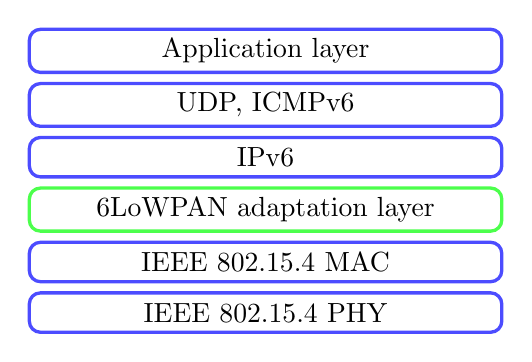
\begin{tikzpicture}[auto]
\begin{scope}
\tikzstyle{layer}=[draw=blue!70,rectangle,rounded corners, minimum width = 6cm, minimum height=5mm, node distance=1mm, very thick]
\tikzstyle{layer2}=[draw=green!70,rectangle,rounded corners, minimum width = 6cm, minimum height=5mm, node distance=1mm, very thick]
\node[layer] (l1) at (0,0) {IEEE 802.15.4 PHY};
\node[layer] (l2) [above=of l1] {IEEE 802.15.4 MAC};
\node[layer2] (l3) [above=of l2] {6LoWPAN adaptation layer};
\node[layer] (l4) [above=of l3] {IPv6};
\node[layer] (l5) [above=of l4] {UDP, ICMPv6};
\node[layer] (l6) [above=of l5] {Application layer};
\end{scope}
\end{tikzpicture}
\caption{6LoWPAN architecture}
\label{stack_6lowpan}
\end{figure}

\subsection{Routing in 6LoWPAN}
In order to address the lack of a routing protocol for 6LoWPAN networks, the RPL protocol has been proposed in RFC 6550 by IETF. Accordingly, RPL provides support for point-to-point (P2P), point-to-multipoint and multipoint-to-point traffic flows \citep{RFC6550}.

The RPL protocol is based on directed acyclic graph (DAG). DAGs are directed graphs formed by a collection of $n$ vertices labeled from the set \{1,2,...,n\}, such that the presence of the edge $(i,j)$ implies that $i < j$. Therefore, each directed edge connects one vertex to another, such that there is no way to start at some vertex $v$ and follow a sequence of edges that eventually loops back to $v$ again \citep{DAGS_1992}. All edges are contained in paths oriented toward and terminating at one or more root nodes. These root nodes are known as Low power and Lossy Network Border Routers (LBR), which are devices that connects the LLN to another routing domain such as a Local Area Network (LAN) or the internet, where a different routing protocol may be in operation. In addition to its functionality as a routing device, the LBR acts as a sink node to a WSN as well as a data collector or aggregator \citep{RFC7102}.

In RPL, a DAG grounded at a single LBR is called a Destination Oriented Directed Acyclic Graph (DODAG). For a specific DODAG, each node is assigned to a rank such that rank increases as the node is far from the LBR. Note that the rank of the nodes along any path to the LBR must be monotonically decreasing, avoiding routing loops, as shown in the figure \ref{RPL_DIO} (each path has a label in this figure, which basically informs the average cost to reach the LBR by a specific parent). Therefore, forwarding a packet to the LBR roughly consist in choosing the neighbor node with the lowest rank.

\begin{figure}[h!tb]
\centering
\ifdefined\TWOCOL
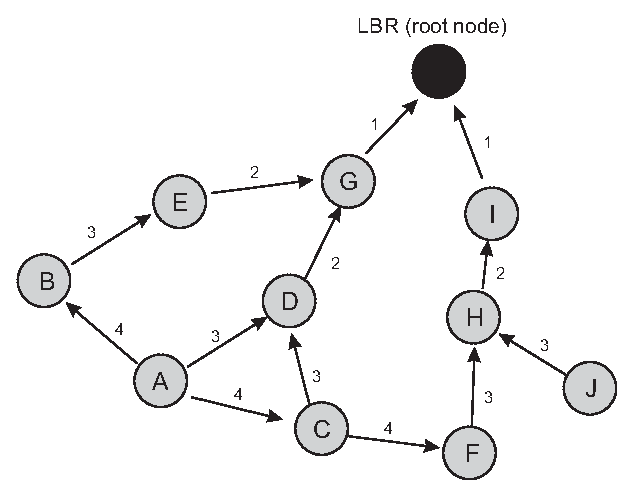
\includegraphics[width=0.45\textwidth]{figures/RPL_DIO}
\else
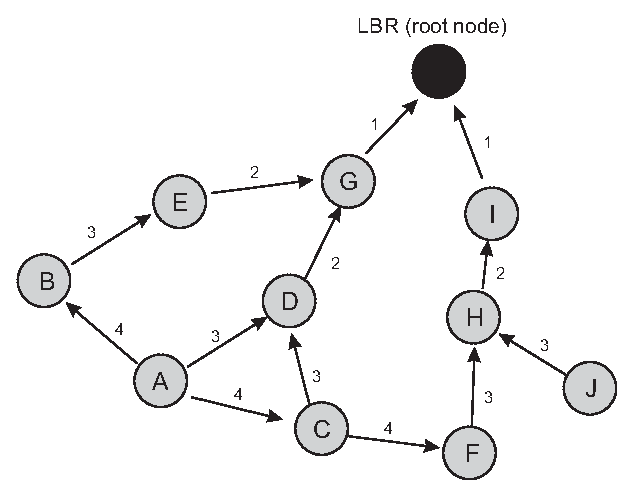
\includegraphics[width=0.8\textwidth]{figures/RPL_DIO}
\fi
\caption{Example of a Destination Oriented Directed Acyclic Graph(DODAG).}
\label{RPL_DIO}
\end{figure}

Nodes running RPL exchange control messages to setup and maintain the DODAG, which in the 6LoWPAN implementation are ICMPv6 messages. The 1 byte code in the ICMPv6 header is used to differentiate between different sub-type of control messages \citep{RFC4443}. The sub-type used to build the DODAG is called DAG Information Object (DIO) \citep{RFC6550}. All the nodes in the network regularly broadcast a DIO to its one-hop neighbors, indicating their activity and rank. The instant at which a node issues a DIO is governed by a Trickle timer \citep{trickle}, which is reset only when an inconsistency arises, i. e., very few DIOs are exchanged when the topology is stable. RPL provides optimized paths to one or more LBRs with very little information stored in the routing table. The information stored is limited to its one-hop neighbors and their parents in the DODAGs. A parent of a node within a DODAG is one of the immediate successors of the node on a path towards the DODAG root.

Despite of its advantages, the default RPL using DODAGs does not provide routes from the LBRs to other nodes in the network, which in RPL are known as down routes. Down refers to the direction from DODAG roots towards leaf nodes, following the reverse direction of DODAG edges. The availability of such routes is desirable in several scenarios, mainly in those with actuators nodes and where selective queries to sensors nodes are required. Thus, a RPL router that requires a path from a LBR to itself should send a DAO (Destination Advertisement Object) message to the LBR through the DODAG edges. The nodes that receive a DAO message forward the message as soon as the timer DelayDAO expires, being this time determined by the implementation, according to \citep{RFC6550}. Therefore, routes for any destination inside the network, other than the LBRs, are provided by these destinations through DAO messages.

The RPL specification defines two modes of operation for the DAO mechanism, storing and non-storing modes. In non-storing mode, each node has to propagate its parent list up to the root. After receiving such topology information, the root computes the path to the destination. Such mode of operating generally makes use of unicast DAO messages to the DODAG root. The storing mode is fully stateful, i.e., each intermediate router in the path towards the root node stores the routes to the destinations in its routing table. To make this possible, each intermediate node adds its downward route to the DAO message, which is unicast to the selected parent(s).

These down routes generated by DAO messages are extremely important to point-to-point communication in the network. An example of the necessity of P2P messages is a scenario where actuators require data from sensors to decide when and how to act. Therefore, if the application needs P2P communication, each pair of nodes must request at least one downward path in order to allow such message exchange. In the worst case, the message is sent from the source router towards the LBR and, thereafter, from the LBR to the destination node, as shown in figure \ref{RPL_DAO}. If the RPL protocol is being performed in the non-storing mode, all point-to-point communication will be conducted by one or more LBRs, which are the only nodes in the network that store downward routes.

\begin{figure}[h!tb]
\centering
\ifdefined\TWOCOL
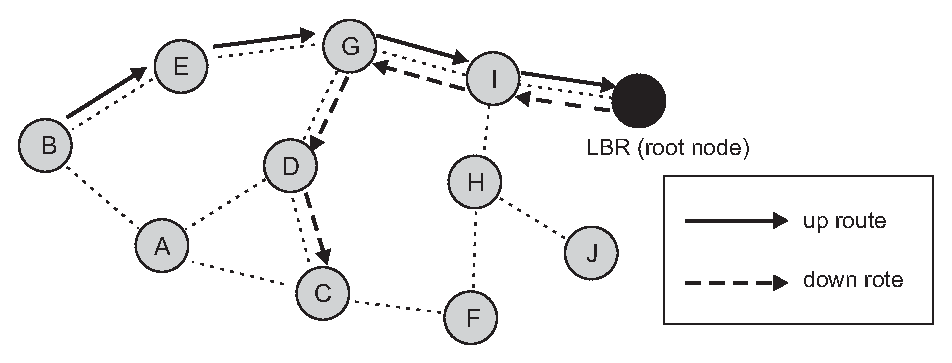
\includegraphics[width=0.45\textwidth]{figures/RPL_DAO}
\else
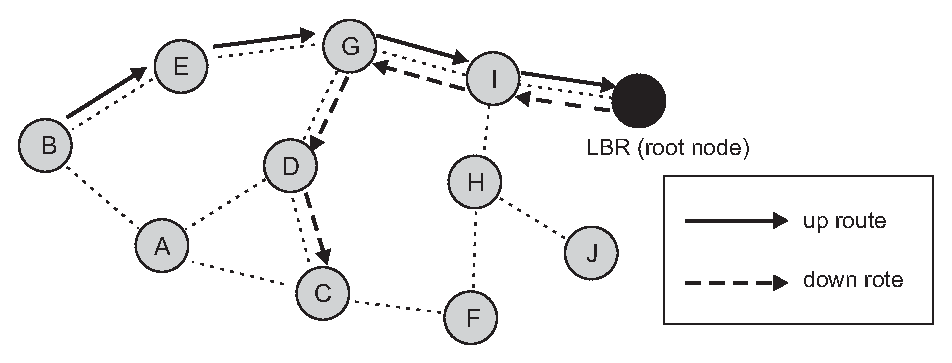
\includegraphics[width=1\textwidth]{figures/RPL_DAO}
\fi
\caption{P2P communication between routers $B$ and $C$ through a DODAG root using RPL.}
\label{RPL_DAO}
\end{figure}

\subsection{Drawbacks of the RPL protocol}

The RPL protocol has several possible drawbacks, depending on the application. Generally, we can point out three usual problems. First, one can easily realize that the P2P routes provided by RPL can be much larger than the shortest available route, causing high traffic on the DODAGs routes (worsening nearby root nodes), as discussed in \citep{P2P_analysis_2010} and \citep{P2P-RPL_2011}. Second, the DAO message exchange may lead to excessive packet collisions, mainly in scenarios with lots of link losses. Thus, the generated downward routes are proactive and initiated by the destination. Therefore, in order for an actuator to make a request to a sensor, the sensor should know that an actuator needs to communicate by point-to-point mode. Third, proactive routing also impacts on the size of the routing table, i.e, the more down routes exists, the greater the memory required to store those paths.

Even, there are problems related to the DAO operating modes. In non-storing mode, RPL requires the use of IPv6 source routing mechanism. Therefore, a Source Routing Header (SRH) for use strictly between RPL routers in the same RPL routing domain was proposed in RFC 6554. However, RPL source routing implements a policy where each IPv6 hop between the source and destination of the source route is specified within the SRH. Such approach leads to a large overhead and increases the consumption of the already scarce bandwidth. Further, as the IEEE 802.15.4 standard has a limited maximum transmission unit (MTU), that may also imply in increased fragmentation. Therefore, successful delivery of an IP packet depends on the successful delivery of all possible fragments, which are not desirable once the LLNs are generally characterized by high packet loss rates.

In addition to the fragmentation issue, the maximum length of the routing header is limited to 255 octets \citep{RFC4944}, which restricts the maximum path length to 127 hops if an address compression mechanism is applied \citep{herberg}. This limitation may exclude scenarios with long chain-like topologies, such as street lighting systems and traffic lights along a street.

In storing mode, each router has to be able to store all the routes downwards its position in the formed DODAGs. This implies that, for routers near to the root node, the required storage is only bounded by the number of paths to all other routers in the network \citep{RPL_observations}. As RPL targets networks consisting of thousands of memory-constrained devices, the required storing capacity on these devices may not be compatible with the basic precepts of the WSANs.

Due to these not negligible drawbacks, it is wise to develop some work around able to improve the RPL protocol deficiencies, mainly that related with P2P messages. To this end, a reactive distance vector routing protocol called LOADng (Lightweight Ad hoc On-Demand - Next Generation (LOADng)) has been proposed \citep{LOADng_2012}. However, in recently published papers (\citep{Tripathi2014, Vucinic_2013}, LOADng was compared to RPL  and, according to the authors, LOADng may even have worse performance than RPL according to several metrics, including average delay, control overhead and maximum memory requirements. Therefore, in this paper, we follow another possible approach for routing. Such approach is the use of geographic routing techniques, which are routing algorithms known by its low overhead and high scalability features \citep{Karp_GPSR_2000, Position_Based_Routing_Ad_Hoc_2001, On_Optimal_Geographic_Routing_2007}.


\section{Geographic Routing}
\label{secGeographicRouting}

Geographic routing mainly relies on a simple greedy geographic forwarding strategy, where each router node must select a locally optimal neighbor with a positive progress towards the data packet destination \citep{survey_2007}. Such approach is largely known by its low overhead and scalability, which can easily be observed due to its low control message system, i.e., a router in a geographic routing strategy only needs to know its direct neighborhood.

In the geographic routing approach, the destination address is the position of the destination node, instead of a topological address. To discover a node position in the network, each router node must implement a location service. This service is responsible to determine its own position and the destination position. A node position could be obtained by pre-configuration if the node is stationary, or by a GPS receiver. \sout{As} \rev{If} network nodes are static \sout{in the street lighting case}, the location information of the nodes can be stored during the installation process. 

When considering realistic outdoor scenarios, such as a city, any block could turn into a void. A void occurs when all neighbors of a router node are farther away from the destination node than the router itself. In this case, the router fails to locate a next hop node through greedy strategy. If only the greedy-forwarding algorithm is used, packets have to be discarded when a void is reached. However, a void does not necessarily mean that there is no route to the destination, because if the network is connected, a valid topological path exists by circumventing the void. 

Many researchers argue that a dense deployment of wireless nodes can reduce the likelihood of the void occurrence in the network \citep{Position_Based_Routing_Ad_Hoc_2001, WSN_routing, survey_2007}. Indeed, in scenarios without obstacles that can be true. However, in outdoor large scale wireless networks it is unlikely to have such scenarios. Void handling techniques is an important issue to be addressed in such networks. 

Among the main non-hybrid void handling techniques, the Greedy Other Adaptive Face Routing (GOAFR) algorithm and its variations is one of the approaches that can get closer to the optimum path when traversing voids \citep{GOAFR_2008}. However, recently some hybrid strategies report having overcome the traditional geographic routing algorithms in terms of hop count, as the Coordinate Depth Forwarding (CDF) technique \citep{Denardin2011}.

Hybrid strategies allow aggregating several techniques in order to achieve better performance than a single technique. In the next section, we propose a hybrid approach that combines the simplicity of the DODAGs routes formed by RPL protocol, the scalability and guaranteed delivery feature of GOAFR algorithm and the inherent optimal paths of the CDF heuristics.

\section{GeoRank}
\label{secGeoRank}

Mainly due to its greedy step, GOAFR algorithm is able to perform quite well in networks with high link density, discovering often optimal or near-optimal paths, in contrast to RPL, which is constrained to route only through the DODAGs and thus, being unable to find the optimal paths. On the other hand, in networks with low link density, mainly around the critical density \citep{GOAFR_2008}, GOAFR has a performance loss and may usually find longer paths than RPL. Therefore, a hybrid approach that leverages the best characteristics of RPL and GOAFR according to the network link density is proposed, resulting in better performance than a single instance of each one would present. The new routing protocol is named \textit{GeoRank} to represent the integration of the geometric based behavior of GOAFR with the rank based behavior of RPL. This approach is mainly suitable for large scale networks with non-uniform link density, such as a wireless network for street lighting nodes, where the link density varies from low to high depending on the presence of obstructions and buildings in different places of the network.

In order to achieve such behavior it is proposed to integrate the CDF technique as a intermediate step in the P2P route algorithm. CDF mainly relies in the hop count towards the base stations (which in terms of RPL are the LBR nodes) to generate suboptimal routes for P2P communication. The basic idea behind such technique is to find the base station closer to the packet destination and, use the optimal path towards such base station (which is based on the hop count metric) to approximate the packet to its destination. However, instead of using directly the hop count to generate the suboptimal paths claimed by CDF, we propose to change its routing metric to the DODAG rank and study its behavior in network topologies based on real street maps. In this way it is possible to use the DODAGs as reliable paths that should be used to accelerate the packet delivery process. The main advantage of using such known and trusted path is to avoid the excessive memory consumption needed by the RPL protocol in order to store the P2P path as well as to reduce the hop count in the GOAFR algorithm around the critical density.

The proposed algorithm obviously depends on geographic position to implement the geometric portion of the protocol. Therefore, all networks nodes must be static, which favors the RPL protocol as well. This does not mean that there must be only static nodes on the network, but that mobile nodes must be one hop away from a static node. As the street lighting system and others possible applications of such network are mainly formed by static devices, it is possible to store the node position during the installation process.

In order to better describe the entire proposed algorithm it is important to define the main principles in which it is based. Therefore, considering a RPL network $G$ comprised of a set $S$ of nodes and a set $B$ of border routers (DODAGs root), we describe the concept of Rank, DODAG preferred parent and DODAG root list.

\begin{mydef}
Rank: Rank $R(u,j)$ is a metric of distance from a given node $u \in S$ to a given DODAG root $j \in B$.
\end{mydef}

The exact way Rank is computed depends on the DAG Objective Function (OF). Even though the specific computation of the Rank is left to the OF, the Rank of the nodes must monotonically decrease as the DODAG is followed towards the DODAG destination.  Therefore, the Rank can be considered a scalar representation of the location or radius of a node within a DODAG.

\begin{mydef}
DODAG Preferred Parent (DPP): Let $u$ be a node of $G$, $N(u)$ its one-hop neighbors and $DPP(u,j)$ a restricted subset of $N(u)$. For each node $v \in N(u)$, $v \in DDP(u,j)$ if it has the lowest rank to reach a specific DODAG root $j \in B$.
\end{mydef}

OBS.: Conceptually, the preferred parent is a single parent. However, it may be a set of multiple parents if those parents are equally preferred and have identical Rank.

\begin{mydef}
DODAG Root List (DRL): each node $v \in N(u)$ should broadcast DIO messages regularly, as previously described. For GeoRank operation, the position of the DODAGs root should be included in such messages. So, let $DRL(j)$ be a list of the DODAGs root position stored in each node $u$ of the network.
\end{mydef}

It is important to note that the proposed algorithm is only intended for down routes. The up routes should use the traditional RPL protocol. Therefore, based on the above definitions, the overall procedure of the \textit{GeoRank} operation is described in Algorithm \ref{alg}.

\small
\begin{algorithm}
\begin{algorithmic}
\caption{GeoRank}
\label{alg}
\small

\STATE \textbf{1. Initialize the algorithm:} Based on the DRL and, the positions of source and destination nodes, trace a line between the source and destination nodes. After, trace lines between the source node and each of the DODAGs root available in the DRL. The DODAG root $j \in DRL$ that has the smallest absolute angle difference to the source-destination line is chosen as a anchor node for the P2P communication. Such anchor node will only be used if the greedy forwarding portion of the GOAFR algorithm fails to deliver the packet. Finally, store the position of the chosen DODAG root $j \in B$ in the packet being forwarded. The angle calculation is better described in \citep{Denardin2011}.

\vspace{2.5mm}

\STATE \textbf{2. Greedy forwarding mode:} If there are one or more neighbors in $N(u)$ closer to the destination than the current node holding the packet $u$, forward the packet to the neighbor $v \in N(u)$ with the greater progress towards the destination. Repeat this approach while such condition exists. If there are no neighbor in such position, store the node $u$ position in the packet and switch to GeoRank mode.

\vspace{2.5mm}

\STATE \textbf{3. GeoRank mode:} If the destination node is closer to the anchor node $j$ (stored in the packet being routed) than the current node holding the packet $u$, forward the packet to the DODAG Preferred Parent $v \in DDP(u,j)$. Repeat such process until : \textbf{a)} the packet reaches a node $u$ whose position is closer to the destination than the position stored in the packet at step 2; \textbf{b)} the packet reach the DODAG root $j$; \textbf{c)} the packet reach the destination node. If condition ``a'' is met, go back to step 2. If condition ``b'' is satisfied, go to step 4.

\vspace{2.5mm}

\STATE \textbf{4. Face routing mode:} Execute face routing mode of GOAFR until: \textbf{a)} delivery the packet; \textbf{b)} the packet reaches a node $u$ whose position is closer to the destination than the position stored in the packet at step 2. If so, go back to step 2.

\small
\end{algorithmic}
\end{algorithm}
\normalsize


\section{Simulation Results}
\label{secSimulation}

In order to evaluate the proposed technique, simulations were performed in scenarios based on real street maps exported from the OpenStreetMap (OSM) data set, which is an open collaborative mapping project \citep{OSM}. The simulator, written in Julia, is based on an idealistic MAC/PHY layer with disc model for radio propagation. The scenarios have been chosen to cover a wide range of possible street layouts inside a square region. They have been populated with nodes with an average distance of $40m$, in order to simulate a real street lighting system, with network sizes ranging from 100 up to 400 nodes. A sample of the chosen scenarios are shown in figure \ref{sim_scenarios}. 

For every scenario, there were generated $1000$ random source-destination pairs, giving a coverage of up to $10$\% of the possible source-destination combinations. For the RPL, the DAG is constructed as the Breadth First Search (BFS) tree for the topology, thus the expected transmission count (ETX) equals one for the preferred parent. Also, every simulation was performed for $10$ random positions of the DODAG root in every scenario, which gives a good coverage of the root placements in a square region, and accounts for the unpredictability in the root location due to several factors, such as the availability of infrastructure (e.g. internet connection),  future network scaling, etc. Then, for the each source-destination pair, the route was determined by each algorithm under test (RPL, GOAFR, \textit{GeoRank} and Dijkstra' algorithm for shortest path) and length of each route was measured in number of hops. The average length of the routes was computed and the results are shown in figure \ref{sim_results} with 95\% confidence intervals. 
  
\begin{figure}
\centering
\ifdefined\TWOCOL
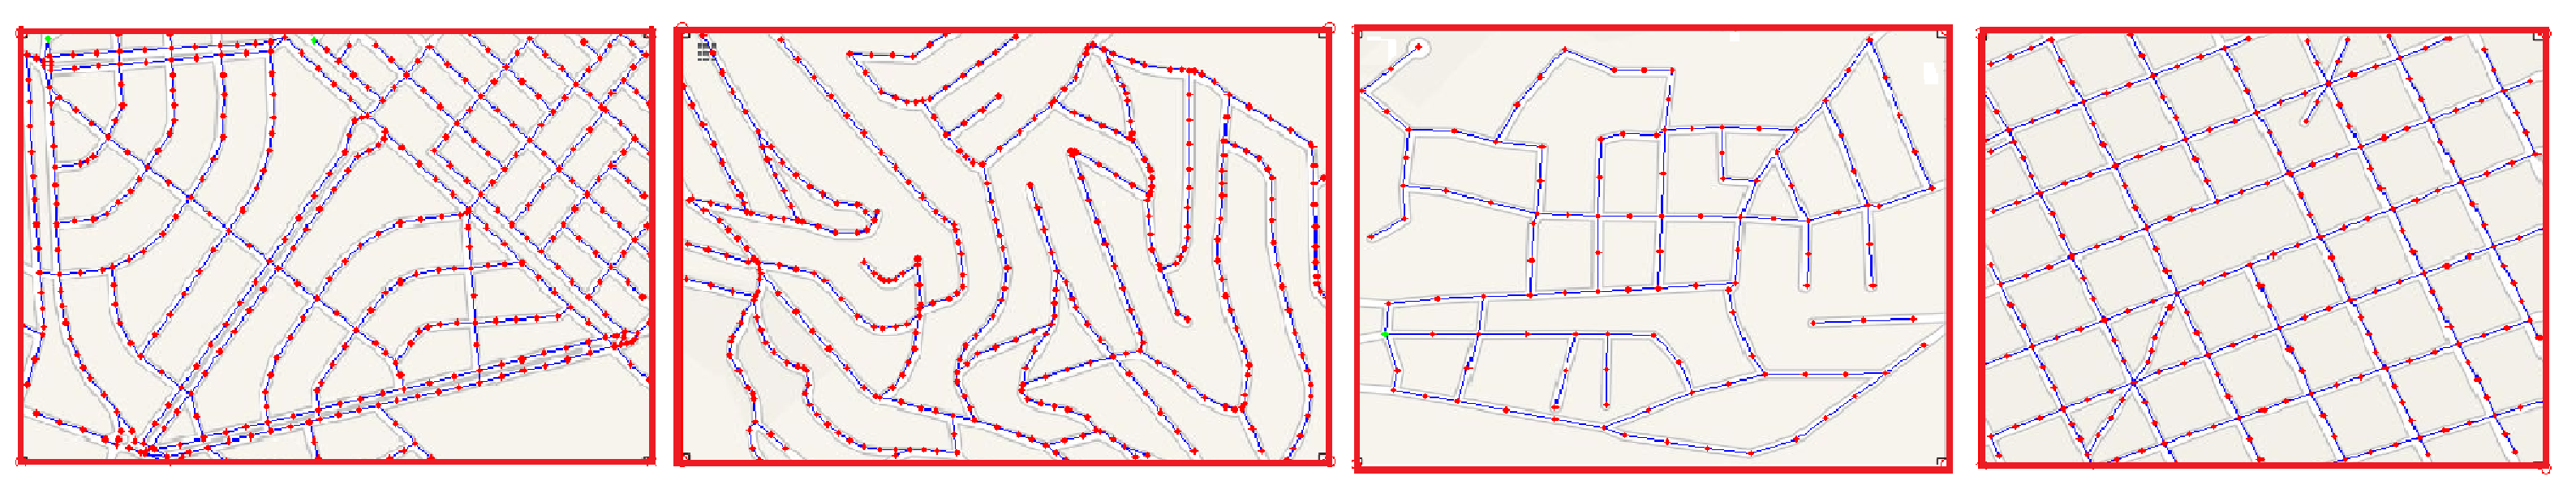
\includegraphics[width=0.45\textwidth]{figures/sample_scenarios.eps}
\else
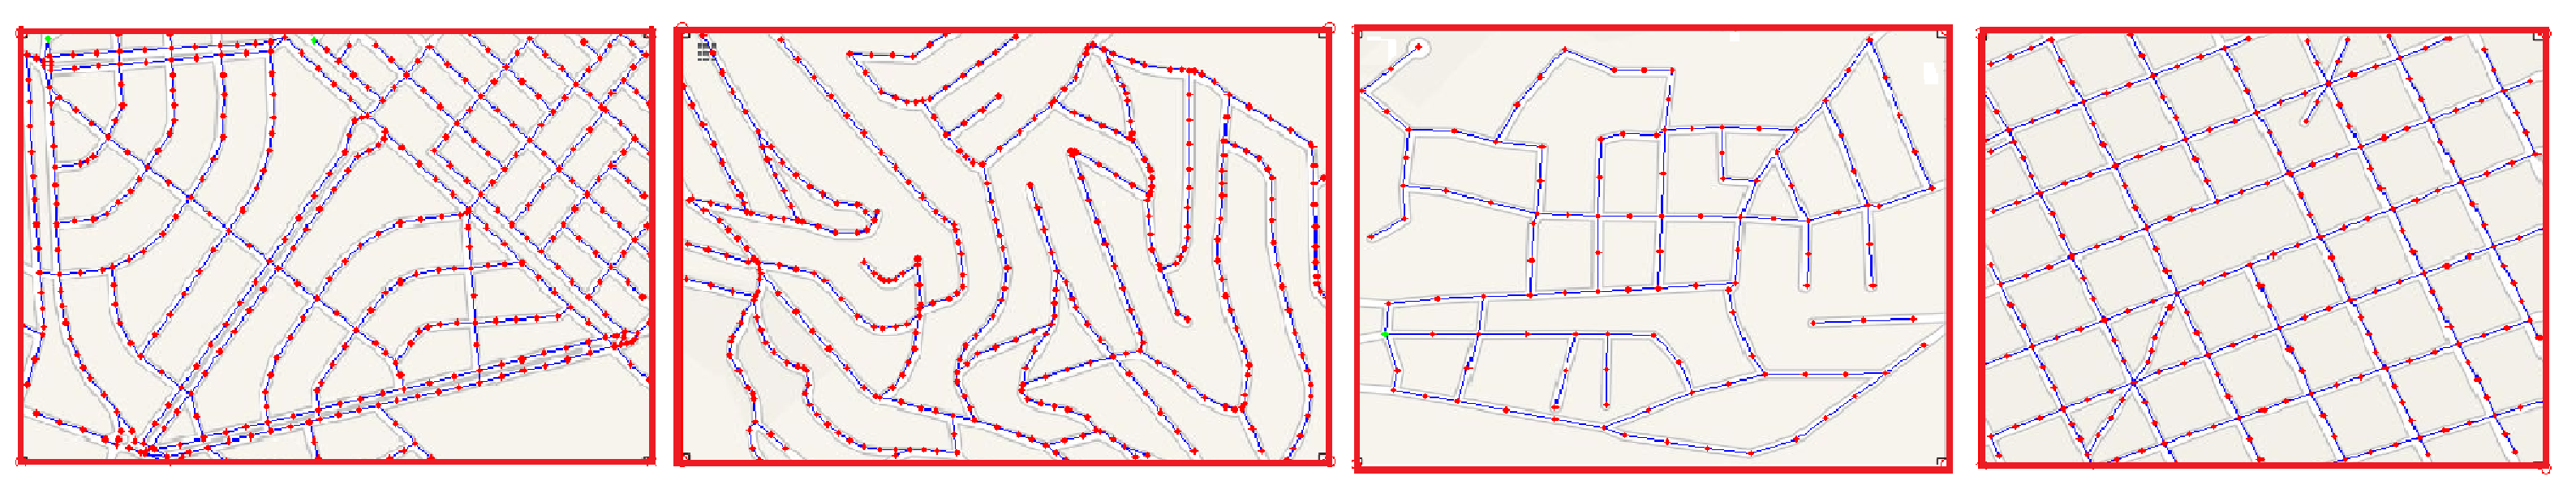
\includegraphics[width=1\textwidth]{figures/sample_scenarios.eps}
\fi
\caption{Sample of simulated scenarios with nodes populated.}
\label{sim_scenarios}
\end{figure}


\begin{figure}
\centering
\ifdefined\TWOCOL
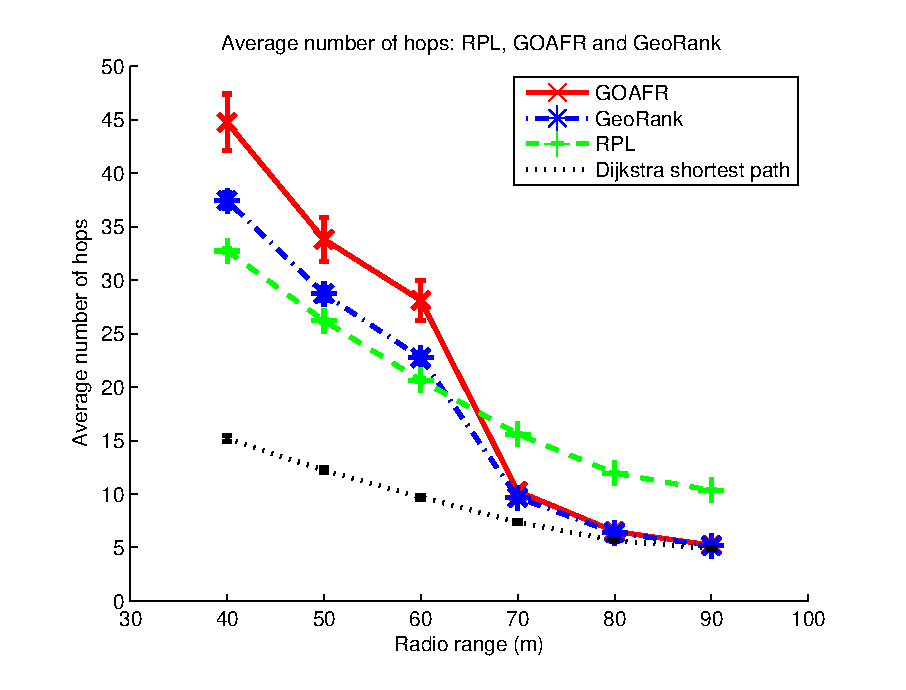
\includegraphics[width=0.45\textwidth]{figures/hops_range.eps}
\else
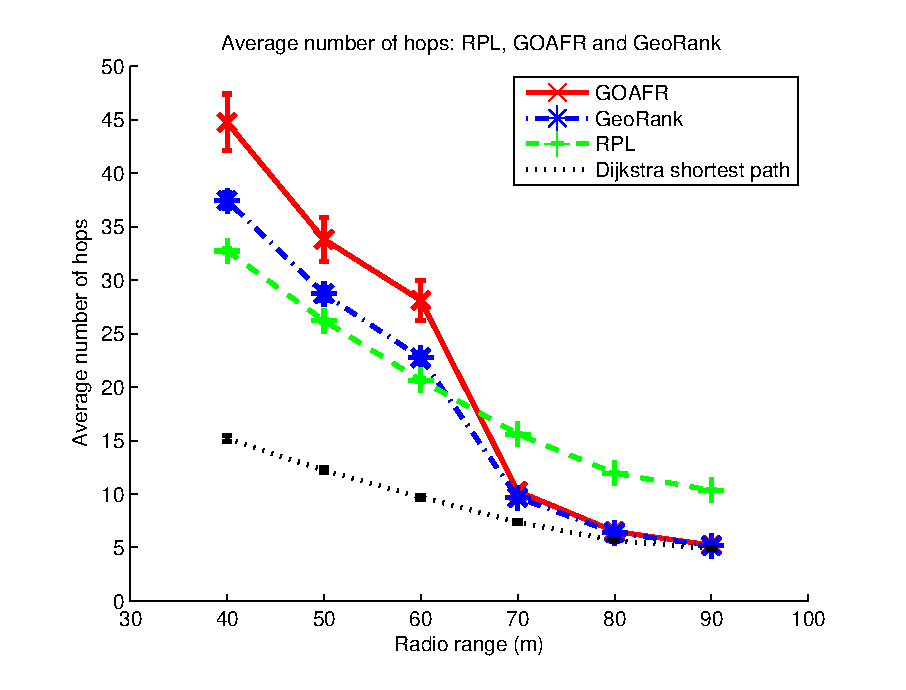
\includegraphics[width=1\textwidth]{figures/hops_range.eps}
\fi
\caption{Simulation results of the average route length for the routing algorithms (RPL, GOAFR, \textit{GeoRank}, and Dijkstra' algorithm for shortest path).}
\label{sim_results}
\end{figure}

For comparison of the scalability of \textit{GeoRank} and RPL, the number of entries in the routing table was recorded for each node. Then, the maximum value of the size of the routing table was computed over all the nodes, because it gives the worst case memory requirement (excluding the DODAG root). The results are shown in figure \ref{sim_results2}.

\begin{figure}
\centering
\ifdefined\TWOCOL
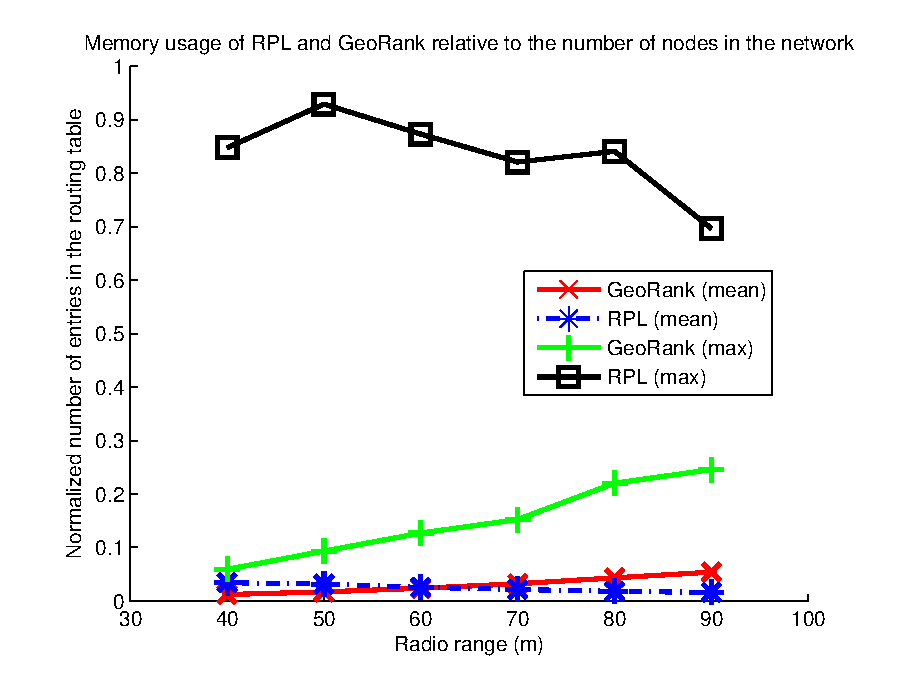
\includegraphics[width=0.45\textwidth]{figures/mem_usage_range.eps}
\else
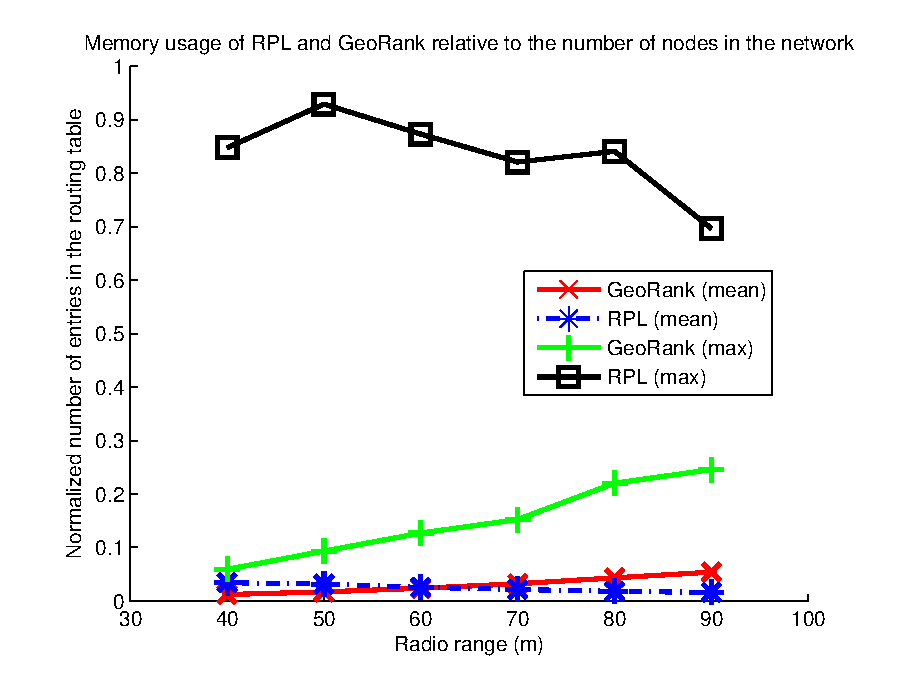
\includegraphics[width=1\textwidth]{figures/mem_usage_range.eps}
\fi
\caption{Simulation results of the size of the routing table in number of entries relative to the number of nodes in the network, for the routing algorithms RPL and \textit{GeoRank}}
\label{sim_results2}
\end{figure}

\subsection{Remarks}

The results shown that, for large radio ranges, where the average connectivity is high, the geographic routing is able to find near optimal routes. The reason for this is that with larger radio ranges the number of links that provide shorter paths are increased and the geographic routing is able to use them for routing, while RPL is constrained to the longer DODAG paths. On the other hand, when the radio range is decreased, the network approaches the critical density, where geographic routing starts to reach more voids in the network and needs to resort more often to the face routing mechanism for circumventing the voids. Thus, the overall effect is that the use of geographic routing results in longer paths than RPL in lower link density conditions.

It is noted that the low link density is the density obtained when the radio range is set to the minimum value required to keep the network connected (i.e. 40m in the simulation setup). And the network is connected when, for any two nodes in the network, there is at least one path connecting them. Also, the high link density is the density obtained when the radio range is set to a value that, for every node in the network, greedy routing always works (i.e. there is no void node). Thus, the packet always is routed through the shortest path in the network (i.e. 90m in the simulation setup).

It is remarkable that the \textit{GeoRank} is able to reduce the length of the route found by geographic routing in lower link densities. It does so by avoiding to circumvent the void with face routing whenever it is possible to use the DODAG to perform this deviation. Thus, \textit{GeoRank} achieves a significant reduction of the path length when the number of voids is large (i.e. when the radio range is small) compared to geographic routing alone. On the other hand, when the radio range is increased, geographic routing performs better than RPL, and \textit{GeoRank} does not impact negatively its performance. Therefore, \textit{GeoRank} works as a selective method, that is able leverage the best of RPL and geographic routing, and being adaptive to the network density.

In a large scale network \sout{, as a smart street lighting}, there may be some places where the link density is very low due to obstacles, such as in dense urban environments, while some places may have high link density due to less and lower buildings. Therefore, while in either case RPL or geographic routing alone would not be the best option, the remarkable adaptability of \textit{GeoRank} makes it the well suited to such variable link density case. Moreover, \textit{GeoRank} is more scalable than storing-mode RPL according to memory usage, as shown in figure \ref{sim_results2}.

\section{Conclusions}
\label{secConclusion}

In this paper, it was proposed a new routing protocol, named \textit{GeoRank}, which integrates the standardized RPL routing protocol for 6LoWPAN networks with the state-of-the-art GOAFR position-based routing algorithm. 
Such a protocol is targeted to be used \sout{in a smart street lighting system based on} \rev{in a large-scale} IPv6-enabled wireless sensor network for supporting diverse applications in an urban IoT. The results obtained from simulations on networks extracted from real street maps have shown that \textit{GeoRank} has an improved routing performance over GOAFR in low link density condition, while outperforming the RPL protocol in high link density condition by finding mostly optimal routes. Therefore, \textit{GeoRank} is an adaptive approach for scenarios with variable link densities. Further, it is remarked that \textit{GeoRank} is not required to use the RPL DAO control messages, because it uses the positions of the nodes for the P2P routing, and is more scalable than storing-mode RPL according to memory usage. 
	
%\section{Acknowledgments}
%\label{secAck}
%
%We thank the OpenStreetMap and its contributors.



%% The Appendices part is started with the command \appendix;
%% appendix sections are then done as normal sections
%% \appendix

%% \label{}

%% References
%%
%% Following citation commands can be used in the body text:
%%
%%  \citet{key}  ==>>  Jones et al. (1990)
%%  \citep{key}  ==>>  (Jones et al., 1990)
%%
%% Multiple citations as normal:
%% \citep{key1,key2}         ==>> (Jones et al., 1990; Smith, 1989)
%%                            or  (Jones et al., 1990, 1991)
%%                            or  (Jones et al., 1990a,b)
%% \cite{key} is the equivalent of \citet{key} in author-year mode
%%
%% Full author lists may be forced with \citet* or \citep*, e.g.
%%   \citep*{key}            ==>> (Jones, Baker, and Williams, 1990)
%%
%% Optional notes as:
%%   \citep[chap. 2]{key}    ==>> (Jones et al., 1990, chap. 2)
%%   \citep[e.g.,][]{key}    ==>> (e.g., Jones et al., 1990)
%%   \citep[see][pg. 34]{key}==>> (see Jones et al., 1990, pg. 34)
%%  (Note: in standard LaTeX, only one note is allowed, after the ref.
%%   Here, one note is like the standard, two make pre- and post-notes.)
%%
%%   \citealt{key}          ==>> Jones et al. 1990
%%   \citealt*{key}         ==>> Jones, Baker, and Williams 1990
%%   \citealp{key}          ==>> Jones et al., 1990
%%   \citealp*{key}         ==>> Jones, Baker, and Williams, 1990
%%
%% Additional citation possibilities
%%   \citeauthor{key}       ==>> Jones et al.
%%   \citeauthor*{key}      ==>> Jones, Baker, and Williams
%%   \citeyear{key}         ==>> 1990
%%   \citeyearpar{key}      ==>> (1990)
%%   \citetext{priv. comm.} ==>> (priv. comm.)
%%   \citenum{key}          ==>> 11 [non-superscripted]
%% Note: full author lists depends on whether the bib style supports them;
%%       if not, the abbreviated list is printed even when full requested.
%%
%% For names like della Robbia at the start of a sentence, use
%%   \Citet{dRob98}         ==>> Della Robbia (1998)
%%   \Citep{dRob98}         ==>> (Della Robbia, 1998)
%%   \Citeauthor{dRob98}    ==>> Della Robbia


%% References with bibTeX database:

\bibliographystyle{bst_models/model2-names}
\bibliography{refs}


%% Authors are advised to submit their bibtex database files. They are
%% requested to list a bibtex style file in the manuscript if they do
%% not want to use model2-names.bst.

%% References without bibTeX database:


% \begin{thebibliography}{00}

%% \bibitem must have one of the following forms:
%%   \bibitem[Jones et al.(1990)]{key}...
%%   \bibitem[Jones et al.(1990)Jones, Baker, and Williams]{key}...
%%   \bibitem[Jones et al., 1990]{key}...
%%   \bibitem[\protect\citeauthoryear{Jones, Baker, and Williams}{Jones
%%       et al.}{1990}]{key}...
%%   \bibitem[\protect\citeauthoryear{Jones et al.}{1990}]{key}...
%%   \bibitem[\protect\astroncite{Jones et al.}{1990}]{key}...
%%   \bibitem[\protect\citename{Jones et al., }1990]{key}...
%%   \harvarditem[Jones et al.]{Jones, Baker, and Williams}{1990}{key}...
%%

% \bibitem[ ()]{}

% \end{thebibliography}

%Carlos Henrique Barriquello is an Adjunct Professor in the Electronics and Computing Department at the Federal University of Santa Maria, Brazil, since 2012. He received the B.Sc., M.Sc. and Ph.D. degrees in electrical engineering from Federal University of Santa Maria in 2007, 2009 and 2012, respectively. His research interests include embedded systems and wireless sensor/actuator networks.

\end{document}

%%
%% End of file `elsarticle-template-2-harv.tex'.
